\documentclass[tikz,border=8pt]{standalone}
% Shared look for every TikZ diagram. Load with % Shared look for every TikZ diagram. Load with % Shared look for every TikZ diagram. Load with \input{../../tools/tikz-style.tex}
\usepackage[T1]{fontenc}
\usepackage{lmodern}
\renewcommand{\sfdefault}{lmr}  % diagrams use the same serif as the text
\usetikzlibrary{arrows.meta, positioning, shapes.geometric, calc, fit, backgrounds}
\definecolor{cblue}{HTML}{4C78A8}
\definecolor{corange}{HTML}{F58518}
\definecolor{cgreen}{HTML}{54A24B}
\definecolor{cred}{HTML}{E45756}
\definecolor{cpurple}{HTML}{B279A2}
\definecolor{cgrey}{HTML}{6B6B6B}
\tikzset{
  every picture/.style={font=\sffamily, line width=1.2pt},
  box/.style={draw=#1, fill=#1!12, rounded corners=4pt, align=center, inner sep=7pt, minimum height=1.1cm},
  box/.default=cgrey,
  arrow/.style={-{Stealth[length=3mm]}, draw=cgrey, line width=1.4pt},
  title/.style={font=\sffamily\bfseries\Large},
  note/.style={font=\sffamily\small, text=cgrey, align=center},
}
\AtBeginDocument{\hyphenpenalty=10000 \exhyphenpenalty=10000}

\usepackage[T1]{fontenc}
\usepackage{lmodern}
\renewcommand{\sfdefault}{lmr}  % diagrams use the same serif as the text
\usetikzlibrary{arrows.meta, positioning, shapes.geometric, calc, fit, backgrounds}
\definecolor{cblue}{HTML}{4C78A8}
\definecolor{corange}{HTML}{F58518}
\definecolor{cgreen}{HTML}{54A24B}
\definecolor{cred}{HTML}{E45756}
\definecolor{cpurple}{HTML}{B279A2}
\definecolor{cgrey}{HTML}{6B6B6B}
\tikzset{
  every picture/.style={font=\sffamily, line width=1.2pt},
  box/.style={draw=#1, fill=#1!12, rounded corners=4pt, align=center, inner sep=7pt, minimum height=1.1cm},
  box/.default=cgrey,
  arrow/.style={-{Stealth[length=3mm]}, draw=cgrey, line width=1.4pt},
  title/.style={font=\sffamily\bfseries\Large},
  note/.style={font=\sffamily\small, text=cgrey, align=center},
}
\AtBeginDocument{\hyphenpenalty=10000 \exhyphenpenalty=10000}

\usepackage[T1]{fontenc}
\usepackage{lmodern}
\renewcommand{\sfdefault}{lmr}  % diagrams use the same serif as the text
\usetikzlibrary{arrows.meta, positioning, shapes.geometric, calc, fit, backgrounds}
\definecolor{cblue}{HTML}{4C78A8}
\definecolor{corange}{HTML}{F58518}
\definecolor{cgreen}{HTML}{54A24B}
\definecolor{cred}{HTML}{E45756}
\definecolor{cpurple}{HTML}{B279A2}
\definecolor{cgrey}{HTML}{6B6B6B}
\tikzset{
  every picture/.style={font=\sffamily, line width=1.2pt},
  box/.style={draw=#1, fill=#1!12, rounded corners=4pt, align=center, inner sep=7pt, minimum height=1.1cm},
  box/.default=cgrey,
  arrow/.style={-{Stealth[length=3mm]}, draw=cgrey, line width=1.4pt},
  title/.style={font=\sffamily\bfseries\Large},
  note/.style={font=\sffamily\small, text=cgrey, align=center},
}
\AtBeginDocument{\hyphenpenalty=10000 \exhyphenpenalty=10000}

\begin{document}
% Section 3: decoder runs for "we're friends ." -> "nous sommes amies . <end>". Training: one run, every position
% computed and used (one loss term each). Inference: 5 runs, each computing every position so far and using only the last.
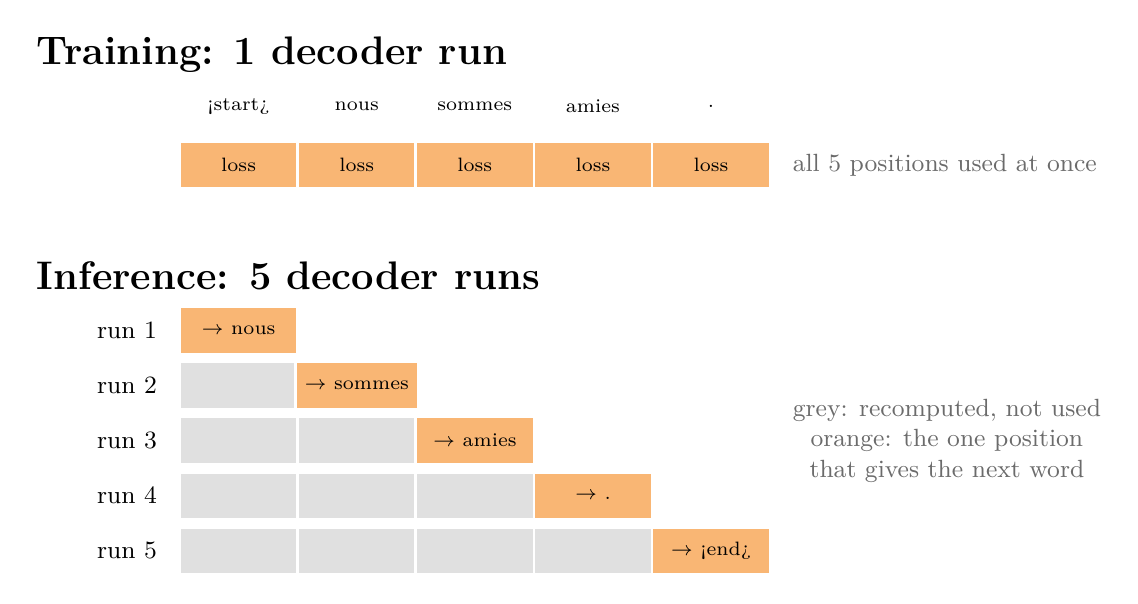
\begin{tikzpicture}[c/.style={draw=white, line width=1pt, minimum width=1.5cm, minimum height=0.6cm, font=\sffamily\scriptsize},
  comp/.style={c, fill=black!12}, used/.style={c, fill=corange!60}]
  \node[title, anchor=west] at (-1.2, 1.4) {Training: 1 decoder run};
  \foreach \w [count=\j] in {<start>, nous, sommes, amies, .} \node[font=\sffamily\scriptsize] at (1.5*\j, 0.75) {\w};
  \foreach \j in {1,...,5} \node[used] at (1.5*\j, 0) {loss};
  \node[note, anchor=west] at (8.4, 0) {all 5 positions used at once};
  \node[title, anchor=west] at (-1.2, -1.4) {Inference: 5 decoder runs};
  \foreach \t/\out in {1/nous, 2/sommes, 3/amies, 4/., 5/{<end>}} {
    \node[font=\sffamily\small, anchor=east] at (0.6, -1.4 - 0.7*\t) {run \t};
    \foreach \j in {1,...,\t} {
      \ifnum\j=\t \node[used] at (1.5*\j, -1.4 - 0.7*\t) {$\to$ \out};
      \else \node[comp] at (1.5*\j, -1.4 - 0.7*\t) {}; \fi
    }
  }
  \node[note, anchor=west] at (8.4, -3.5) {grey: recomputed, not used\\orange: the one position\\that gives the next word};
\end{tikzpicture}
\end{document}
